\item \subquestionpoints{3} {\bf Coding question: degree-3 polynomial regression}


For this sub-question question, we will use the dataset provided in
the following files:
%
\begin{center}
	\url{src/featuremaps/{train,valid,test}.csv}
\end{center}
%

Each file contains two columns: $x$ and $y$. In the terminology described in the introduction, $x$ is the attribute (in this case one dimensional) and $y$ is the output label.

Using the formulation of the previous sub-question, implement linear regression with \textbf{normal equations} using the feature map of degree-3 polynomials. Use the starter code provided in \texttt{src/featuremaps/featuremap.py} to implement the algorithm.

Create a scatter plot of the training data, and plot the learnt hypothesis as a smooth curve over it. Submit the plot in the writeup as the solution for this problem.

\emph{Remark: } Suppose $\widehat{X}$ is the design matrix of the transformed dataset. You may sometimes encounter a non-invertible matrix $\widehat{X}^T\widehat{X}$. For a numerically stable code implementation, always use \texttt{np.linalg.solve} to obtain the parameters directly, rather than explicitly calculating the inverse and then multiplying it with $\widehat{X}^Ty$.\\

Your plot should look similar to the following:
\begin{figure}[H]
  \centering
  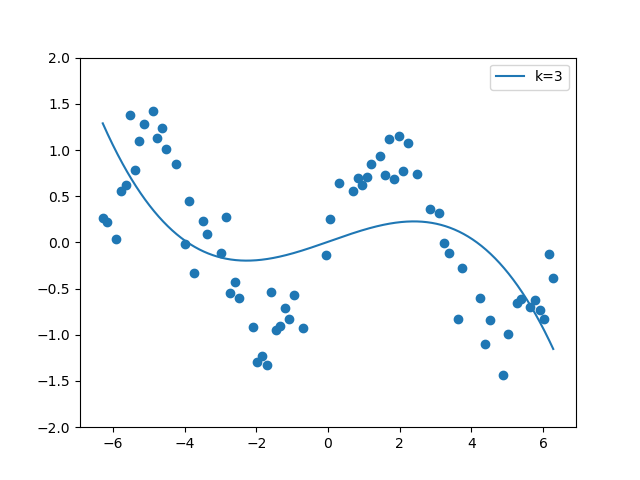
\includegraphics[width=0.65\linewidth]{featuremaps/src/large-poly3.png}
  \centering
\caption{Polynomial regression with degree 3}
\end{figure}
